\documentclass[../master/master.tex]{subfiles}

\begin{document}

%----------------------------------------------------------------------
% LECTURE 5: Compactness, Perfect Sets
% Date: February 3, 2026
%----------------------------------------------------------------------
\renewcommand{\lecturenum}{5}
\renewcommand{\lecturedate}{February 3, 2026}
\renewcommand{\lecturetopic}{Compactness, Perfect Sets}

\section{Lecture \lecturenum : \lecturedate}

\subsection{Compactness}

\begin{definition}
Let $E \subseteq X$ be a topological space. If $\{G_\alpha\}$ is a collection of open sets of $X$ such that $E \subseteq \bigcup G_\alpha$, then $\{G_\alpha\}$ is an \defn{open cover} of $E$.
\end{definition}

\begin{definition}
A subset $K \subseteq X$ is \defn{compact} if every open cover contains a finite subcover. That is, given $\{G_\alpha\}$, there exist $G_{\alpha_1}, \dots, G_{\alpha_n} \subseteq \{G_\alpha\}$ such that $K \subseteq G_{\alpha_1} \cup G_{\alpha_2} \cup \cdots \cup G_{\alpha_n}$.
\end{definition}

\begin{notebox}
\textbf{Understanding covers and compactness.} An open cover is a collection of open sets that together contain every point of $E$. Think of it as ``blanketing'' the set with open sets. The cover may have infinitely many sets --- in fact, that's the interesting case.

Compactness says: no matter how you cover $K$ with open sets, you can always throw away all but finitely many and still cover $K$. This is a strong condition --- it fails for many sets.

\begin{center}
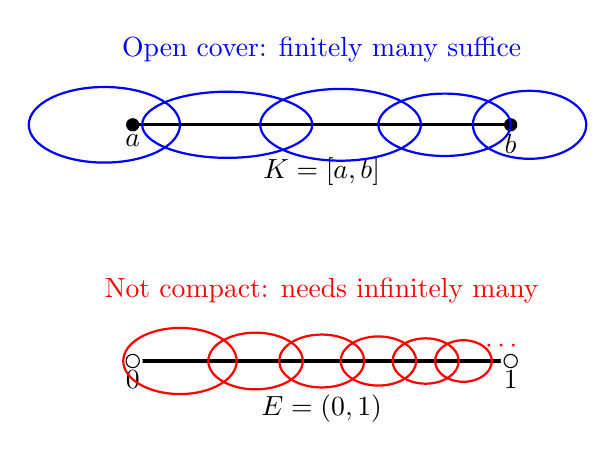
\begin{tikzpicture}[scale=1.2]
    % Compact set (closed interval)
    \draw[very thick] (0,0) -- (4,0);
    \fill (0,0) circle (2pt) node[below] {$a$};
    \fill (4,0) circle (2pt) node[below] {$b$};
    \node at (2, -0.5) {$K = [a,b]$};

    % Open cover - several overlapping open sets
    \draw[blue, thick] (-0.3, 0) ellipse (0.8 and 0.4);
    \draw[blue, thick] (1, 0) ellipse (0.9 and 0.35);
    \draw[blue, thick] (2.2, 0) ellipse (0.85 and 0.38);
    \draw[blue, thick] (3.3, 0) ellipse (0.7 and 0.33);
    \draw[blue, thick] (4.2, 0) ellipse (0.6 and 0.36);

    \node[blue] at (2, 0.8) {Open cover: finitely many suffice};

    % Non-compact set
    \begin{scope}[yshift=-2.5cm]
        \draw[very thick] (0,0) -- (4,0);
        \fill[white] (0,0) circle (3pt);
        \draw (0,0) circle (2pt) node[below] {$0$};
        \fill[white] (4,0) circle (3pt);
        \draw (4,0) circle (2pt) node[below] {$1$};
        \node at (2, -0.5) {$E = (0,1)$};

        % Infinitely many covers needed
        \draw[red, thick] (0.5, 0) ellipse (0.6 and 0.35);
        \draw[red, thick] (1.3, 0) ellipse (0.5 and 0.3);
        \draw[red, thick] (2, 0) ellipse (0.45 and 0.28);
        \draw[red, thick] (2.6, 0) ellipse (0.4 and 0.26);
        \draw[red, thick] (3.1, 0) ellipse (0.35 and 0.24);
        \draw[red, thick] (3.5, 0) ellipse (0.3 and 0.22);
        \node[red] at (3.9, 0.15) {$\cdots$};

        \node[red] at (2, 0.75) {Not compact: needs infinitely many};
    \end{scope}
\end{tikzpicture}
\end{center}

The closed interval $[a,b]$ is compact: any open cover has a finite subcover. The open interval $(0,1)$ is not compact: the cover $\{(\frac{1}{n}, 1) : n \geq 2\}$ has no finite subcover, since points near $0$ escape any finite subcollection.
\end{notebox}

\subsection{Subspace Topology}

$Y \subseteq X$. $U$ is open in $Y$ if and only if there exists $V$ open in $X$ such that $U = V \cap Y$.

\begin{theorem}
If $K \subseteq Y \subseteq X$, then $K$ compact relative to $X$ $\Leftrightarrow$ $K$ compact relative to $Y$.
\end{theorem}

\begin{proof}
$(\Rightarrow)$ Suppose $K$ is compact relative to $X$. Let $\{U_\alpha\}$ be an open cover of $K$ in $Y$. By the subspace topology, for each $U_\alpha$ there exists $V_\alpha$ open in $X$ such that $U_\alpha = V_\alpha \cap Y$. Then $\{V_\alpha\}$ is an open cover of $K$ in $X$. Since $K$ is compact relative to $X$, there exist $V_{\alpha_1}, \dots, V_{\alpha_n}$ such that $K \subseteq V_{\alpha_1} \cup \cdots \cup V_{\alpha_n}$. Then
\[
K \subseteq (V_{\alpha_1} \cup \cdots \cup V_{\alpha_n}) \cap Y = U_{\alpha_1} \cup \cdots \cup U_{\alpha_n}.
\]
So $K$ is compact relative to $Y$.

$(\Leftarrow)$ Suppose $K$ is compact relative to $Y$. Let $\{V_\alpha\}$ be an open cover of $K$ in $X$. Then $\{V_\alpha \cap Y\}$ is an open cover of $K$ in $Y$ (each $V_\alpha \cap Y$ is open in $Y$ by the subspace topology). Since $K$ is compact relative to $Y$, there exist $V_{\alpha_1} \cap Y, \dots, V_{\alpha_n} \cap Y$ such that $K \subseteq (V_{\alpha_1} \cap Y) \cup \cdots \cup (V_{\alpha_n} \cap Y)$. Since $K \subseteq Y$, we have $K \subseteq V_{\alpha_1} \cup \cdots \cup V_{\alpha_n}$. So $K$ is compact relative to $X$.
\end{proof}

\begin{theorem}
Compact subsets of metric spaces are closed.
\end{theorem}

\begin{proof}
It suffices to show that $K^c$ is open. Since we are in a metric space, we can use the open ball definition of open sets. We will show for every point $p \in K^c$, there exists $\eps > 0$ such that $B(p, \eps) \subseteq K^c$.

Fix $p \in K^c$. For each $q \in K$, let $r_q = \frac{1}{2}d(p, q) > 0$. The balls $B(p, r_q)$ and $B(q, r_q)$ are disjoint. The collection $\{B(q, r_q) : q \in K\}$ is an open cover of $K$. By compactness, there exist $q_1, \dots, q_n \in K$ such that
\[
K \subseteq B(q_1, r_{q_1}) \cup \cdots \cup B(q_n, r_{q_n}).
\]
Let $\eps = \min(r_{q_1}, \dots, r_{q_n}) > 0$. Then $B(p, \eps) \subseteq K^c$, since $B(p, \eps) \subseteq B(p, r_{q_i})$ is disjoint from $B(q_i, r_{q_i})$ for each $i$, and $K$ is covered by these balls.
\end{proof}

\begin{theorem}
Closed subsets of compact sets are compact.
\end{theorem}

\begin{proof}
Let $F$ be a closed subset of a compact set $K$ in $X$. Let $\{G_\alpha\}$ be an open cover of $F$. Then $\{G_\alpha\} \cup \{F^c\}$ is an open cover of $K$ ($F$ is closed so $F^c$ is open, and $\{G_\alpha\}$ covers $F$). Since $K$ is compact, there exists a finite subcover: $G_{\alpha_1}, \dots, G_{\alpha_n}$, and possibly $F^c$. Removing $F^c$ (if present), we have $F \subseteq G_{\alpha_1} \cup \cdots \cup G_{\alpha_n}$. Thus $F$ is compact.
\end{proof}

\begin{corollary}
The intersection of a closed set and a compact set is compact (in a metric space).
\end{corollary}

\begin{theorem}
Suppose $\{K_\alpha\}$ is a collection of compact subsets of a metric space $X$ such that the intersection of any finite subcollection is nonempty. Then $\bigcap_\alpha K_\alpha \neq \emptyset$.
\end{theorem}

\begin{proof}
Suppose $\bigcap_\alpha K_\alpha = \emptyset$. Each $K_\alpha^c$ is open. By De Morgan's law,
\[
\left(\bigcap_\alpha K_\alpha\right)^c = \bigcup_\alpha K_\alpha^c = X.
\]
Fix $K_1 \in \{K_\alpha\}$. Then $\{K_\alpha^c\}$ is an open cover of $K_1$. By compactness, there exist $K_{\alpha_1}, \dots, K_{\alpha_n}$ such that $K_1 \subseteq K_{\alpha_1}^c \cup \cdots \cup K_{\alpha_n}^c$. By De Morgan's law,
\[
K_1 \subseteq \left(K_{\alpha_1} \cap \cdots \cap K_{\alpha_n}\right)^c.
\]
Thus $K_1 \cap K_{\alpha_1} \cap \cdots \cap K_{\alpha_n} = \emptyset$, contradicting the finite intersection property.
\end{proof}

\begin{corollary}
If $\{K_n\}$ is a sequence of compact subsets of a metric space $X$ such that $K_n \supseteq K_{n+1}$, then $\bigcap_n K_n \neq \emptyset$.
\end{corollary}

\begin{theorem}
If $E$ is an infinite subset of a compact set $K$, then $E$ has a limit point in $K$.
\end{theorem}

\begin{proof}
(By contradiction) Assume that $E$ has no limit points. Then for all $p \in K$, there exists a neighborhood $U_p$ of $p$ where either $U_p \cap E = \emptyset$ or $U_p \cap E = \{p\}$. Therefore, $\{U_p\}$ forms an open cover of $K$. By compactness of $K$, there is a finite subcover $U_{p_1} \cup \cdots \cup U_{p_n} \supseteq K$. Each $U_{p_i}$ contains at most one point of $E$, so $E$ has at most $n$ points. This contradicts the fact that $E$ is infinite.
\end{proof}

\begin{notebox}
\textbf{The Cantor set is nonempty.} Recall the Cantor set is defined as $C = \bigcap_{n=0}^{\infty} C_n$, where each $C_n$ is a finite union of closed intervals. Each $C_n$ is compact. The sets are nested: $C_0 \supseteq C_1 \supseteq C_2 \supseteq \cdots$, so any finite intersection equals the smallest set in the subcollection, which is nonempty. By the theorem above, $C = \bigcap_{n=0}^{\infty} C_n \neq \emptyset$.
\end{notebox}

\begin{theorem}
Suppose $\{I_n\}$ is a sequence of closed intervals in $\R$ such that $I_n \supseteq I_{n+1}$. Then $\bigcap_k I_k \neq \emptyset$.
\end{theorem}

\begin{proof}
Let $I_n = [a_n, b_n]$. Let $E = \{a_n\}$. Since the intervals are nested, $a_n \leq b_m$ for all $n, m$, so $E$ is bounded above. There exists $x = \sup E$.

For all $n$, we have $a_n \leq x$ (since $x$ is an upper bound of $E$). Also $x \leq b_n$ for all $n$ (since each $b_n$ is an upper bound for $E$, and $x$ is the least upper bound). Thus $a_n \leq x \leq b_n$, so $x \in I_n$ for all $n$. Therefore $x \in \bigcap_k I_k$.
\end{proof}

\begin{theorem}
Closed intervals (and therefore closed boxes) are compact.
\end{theorem}

\begin{proof}
Let $I = [a, b]$ and let $\{G_\alpha\}$ be an open cover of $I$. Suppose this open cover does not reduce to a finite subcover. Cut the interval in half: at least one half cannot be covered by finitely many $G_\alpha$ (if both halves could, we could combine them to cover $I$). Call this half $I_1$. Repeat: bisect $I_1$ and choose a half $I_2$ with no finite subcover. Continuing, we obtain nested closed intervals $I \supseteq I_1 \supseteq I_2 \supseteq \cdots$ with $|I_n| = (b-a)/2^n$, each having no finite subcover.

By the nested intervals theorem, there exists $x \in \bigcap_n I_n$. Since $\{G_\alpha\}$ covers $I$, we have $x \in G_\alpha$ for some $\alpha$. Since $G_\alpha$ is open, there exists $\eps > 0$ such that $(x - \eps, x + \eps) \subseteq G_\alpha$. For large $n$, $|I_n| < \eps$ and $x \in I_n$, so $I_n \subseteq (x - \eps, x + \eps) \subseteq G_\alpha$. But then $I_n$ is covered by a single open set, contradicting that $I_n$ has no finite subcover.

\begin{center}
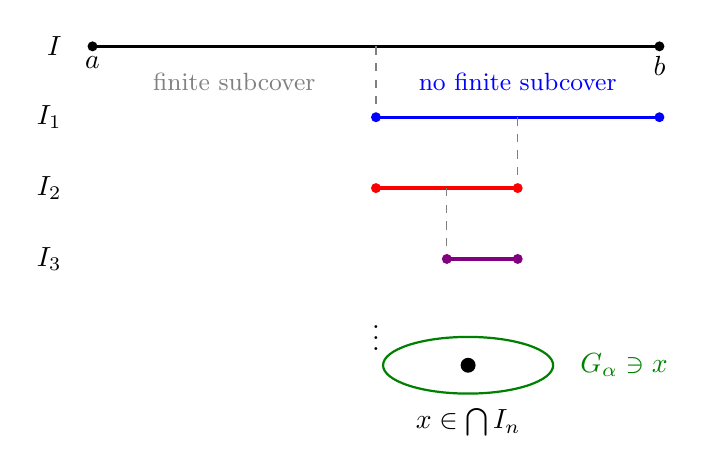
\begin{tikzpicture}[scale=0.9]
    % Original interval
    \draw[very thick] (0,0) -- (8,0);
    \fill (0,0) circle (2pt) node[below] {$a$};
    \fill (8,0) circle (2pt) node[below] {$b$};
    \node[left] at (-0.3,0) {$I$};

    % First bisection
    \draw[very thick, blue] (4,-1) -- (8,-1);
    \draw[dashed, gray] (4,0) -- (4,-1);
    \fill[blue] (4,-1) circle (2pt);
    \fill[blue] (8,-1) circle (2pt);
    \node[left] at (-0.3,-1) {$I_1$};
    \node[gray] at (2,-0.5) {\small finite subcover};
    \node[blue] at (6,-0.5) {\small no finite subcover};

    % Second bisection
    \draw[very thick, red] (4,-2) -- (6,-2);
    \draw[dashed, gray] (6,-1) -- (6,-2);
    \fill[red] (4,-2) circle (2pt);
    \fill[red] (6,-2) circle (2pt);
    \node[left] at (-0.3,-2) {$I_2$};

    % Third bisection
    \draw[very thick, violet] (5,-3) -- (6,-3);
    \draw[dashed, gray] (5,-2) -- (5,-3);
    \fill[violet] (5,-3) circle (2pt);
    \fill[violet] (6,-3) circle (2pt);
    \node[left] at (-0.3,-3) {$I_3$};

    % Limit point
    \node at (4,-4) {$\vdots$};
    \fill[black] (5.3,-4.5) circle (3pt);
    \node at (5.3,-5.3) {$x \in \bigcap I_n$};

    % Open set containing x
    \draw[thick, green!50!black] (5.3,-4.5) ellipse (1.2 and 0.4);
    \node[green!50!black] at (7.5,-4.5) {$G_\alpha \ni x$};
\end{tikzpicture}
\end{center}
\end{proof}

\begin{notebox}
\textbf{Key ideas in this proof:}
\begin{enumerate}
    \item \textbf{Proof by contradiction:} Assume no finite subcover exists and derive a contradiction.
    \item \textbf{Bisection argument:} If a set has no finite subcover, at least one half doesn't either. This lets us build nested intervals.
    \item \textbf{Nested intervals theorem:} The intersection $\bigcap I_n \neq \emptyset$, giving us a point $x$.
    \item \textbf{Open set definition:} Since $x \in G_\alpha$ and $G_\alpha$ is open, there exists $\eps > 0$ with $(x - \eps, x + \eps) \subseteq G_\alpha$.
    \item \textbf{Intervals shrink to zero:} $|I_n| = (b-a)/2^n \to 0$, so eventually $I_n$ fits inside the $\eps$-neighborhood, giving a single-set cover --- contradiction.
\end{enumerate}
\end{notebox}

\newpage

\begin{theorem}[\defn{Heine-Borel}]
Let $E \subseteq \R^n$. The following are equivalent:
\begin{enumerate}
    \item $E$ is closed and bounded.
    \item $E$ is compact.
    \item Every infinite subset of $E$ has a limit point in $E$.
\end{enumerate}
\end{theorem}

\begin{proof}
$(1 \Rightarrow 2)$: Since $E$ is bounded, $E \subseteq [-M, M]^n$ for some $M > 0$. The closed box $[-M, M]^n$ is compact. Since $E$ is a closed subset of a compact set, $E$ is compact.

$(2 \Rightarrow 3)$: This follows from the theorem: if $E$ is an infinite subset of a compact set $K$, then $E$ has a limit point in $K$. Taking $K = E$, every infinite subset of $E$ has a limit point in $E$.

$(3 \Rightarrow 1)$:
\textit{Closed:} Let $p$ be a limit point of $E$. Every neighborhood of $p$ contains a point of $E$ distinct from $p$. We can construct a sequence $(x_n)$ in $E$ with $x_n \to p$. The set $\{x_n\}$ is infinite, so by (3) it has a limit point in $E$. This limit point must be $p$, so $p \in E$. Thus $E$ contains all its limit points, so $E$ is closed.

\textit{Bounded:} Suppose $E$ is unbounded. Then for each $n \in \N$, there exists $x_n \in E$ with $|x_n| > n$. The set $\{x_1, x_2, \dots\}$ is infinite. By (3), it has a limit point $p \in E$. But for any $\eps > 0$, only finitely many $x_n$ lie in $B(p, \eps)$ (since $|x_n| \to \infty$), contradicting that $p$ is a limit point. Thus $E$ is bounded.
\end{proof}

\begin{notebox}
\textbf{What Heine-Borel means and how to use it.}

In $\R^n$, compactness has a simple characterization: \textit{closed and bounded}. This is easy to check! You don't need to verify that every open cover has a finite subcover --- just check two conditions.

\textbf{Common uses:}
\begin{itemize}
    \item \textbf{Proving a set is compact:} Show it's closed (contains its limit points) and bounded (fits in some ball). Examples: $[0,1]$, closed balls $\overline{B}(x, r)$, the Cantor set.
    \item \textbf{Proving a set is NOT compact:} Show it's either not closed or not bounded. Examples: $(0,1)$ is not closed; $\R$ is not bounded.
    \item \textbf{Extracting convergent subsequences:} Condition (3) says infinite subsets have limit points. This is the key to proving the Bolzano-Weierstrass theorem: every bounded sequence in $\R^n$ has a convergent subsequence.
\end{itemize}

\textbf{Warning:} Heine-Borel is specific to $\R^n$. In general metric spaces, compact implies closed and bounded, but the converse can fail.
\end{notebox}

\begin{theorem}[\defn{Weierstrass}]
Every bounded infinite subset has a limit point in $\R^n$.
\end{theorem}

\subsection{Perfect Sets}

Recall: $E$ is \defn{perfect} if $E$ is closed and has no isolated points. If $E$ is perfect, then $E = \overline{E} = E'$.

\begin{theorem}
Every nonempty perfect subset of $\R^n$ is uncountable.
\end{theorem}

\begin{proof}
Let $P \subseteq \R^n$ be nonempty and perfect. Suppose for contradiction that $P$ is countable, say $P = \{x_1, x_2, x_3, \dots\}$.

We construct nested closed sets $V_1 \supseteq V_2 \supseteq V_3 \supseteq \cdots$ such that:
\begin{enumerate}
    \item $V_n \cap P \neq \emptyset$ for all $n$,
    \item $x_n \notin V_n$ for all $n$.
\end{enumerate}

\textbf{Base case:} Since $P$ has no isolated points, $x_1$ is a limit point of $P$. Choose $y_1 \in P$ with $y_1 \neq x_1$. Let $V_1 = \overline{B}(y_1, r_1)$ where $r_1 = \frac{1}{2}d(x_1, y_1)$. Then $y_1 \in V_1 \cap P$ and $x_1 \notin V_1$.

\textbf{Inductive step:} Suppose $V_n$ is constructed with $V_n \cap P \neq \emptyset$ and $x_n \notin V_n$. Pick any $y \in V_n \cap P$. Since $P$ is perfect, $y$ is a limit point of $P$, so there exists $y_{n+1} \in P \cap V_n$ with $y_{n+1} \neq x_{n+1}$ (if $x_{n+1} \notin V_n$, any point works; if $x_{n+1} \in V_n$, choose a different point). Let $V_{n+1} = \overline{B}(y_{n+1}, r_{n+1}) \cap V_n$ where $r_{n+1}$ is small enough that $x_{n+1} \notin V_{n+1}$ and $V_{n+1} \subseteq V_n$.

Each $V_n$ is closed and bounded, hence compact. The $V_n$ are nested and nonempty, so by the finite intersection property, $\bigcap_n V_n \neq \emptyset$. Let $x \in \bigcap_n V_n$. Since each $V_n \cap P$ is closed (intersection of closed sets) and the $V_n$ are nested, we have $x \in P$. But $x \neq x_n$ for all $n$ (since $x_n \notin V_n$). This contradicts $P = \{x_1, x_2, \dots\}$.
\end{proof}

\begin{theorem}
The Cantor set is perfect.
\end{theorem}

\begin{proof}
The Cantor set $C$ is closed. Additionally, using the ternary expansion: for any $x \in C$, we can truncate $x$ at the $n$-th digit and define a sequence $(x_n)$ in $C$ with $|x - x_n| \leq 3^{-n}$. Thus $x_n \to x$, so $x$ is a limit point of $C$. Hence $C$ has no isolated points, and $C$ is perfect.

\begin{center}
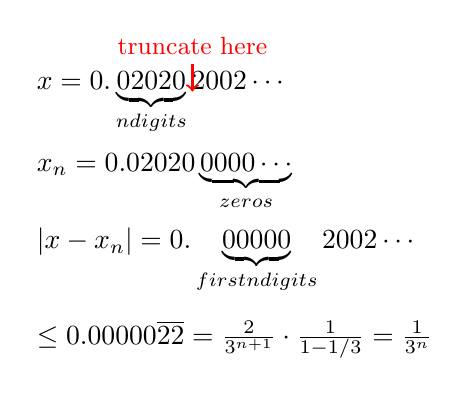
\begin{tikzpicture}
    % Original number
    \node[anchor=west] at (0, 0) {$x = 0.\underbrace{0 2 0 2 0}_{n \text{ digits}} 2 0 0 2 \cdots$};

    % Truncated number
    \node[anchor=west] at (0, -1) {$x_n = 0.0 2 0 2 0 \underbrace{0 0 0 0 \cdots}_{\text{zeros}}$};

    % Difference
    \node[anchor=west] at (0, -2) {$|x - x_n| = 0.\underbrace{0 0 0 0 0}_{\text{first } n \text{ digits}} 2 0 0 2 \cdots$};

    % Bound
    \node[anchor=west] at (0, -3) {$\leq 0.00000\overline{22} = \frac{2}{3^{n+1}} \cdot \frac{1}{1 - 1/3} = \frac{1}{3^n}$};

    % Arrow showing truncation point
    \draw[->, thick, red] (2.1, 0.5) -- (2.1, 0.15);
    \node[red, above] at (2.1, 0.5) {\small truncate here};
\end{tikzpicture}
\end{center}
\end{proof}

\end{document}
